\chapter{Our Approach}
\label{sec:our-approach}

\section{System Architecture}
% Brief introdcution of all actors, components and messages
% The specification is complicated because it is the result of long discussions and a clarification process (See https://project.redbackup.org/browse/REDPRO-98)
% See Describing architectures in https://wiki.hsr.ch/FarhadMehta/files/Writing_Scientific_Papers.pdf
% Describe everything concise and with exact definitions.
% Use schemes and flowcharts

There are two kinds of actors interacting with the system. A typical \gls{user} wants to store backups in the redbackup system and restore them (partially) when needed. The other kind of actor is an \gls{administrator} that configures the system, e.g. extends storage capacity or replaces corrupted disks. Distinctive for both actors is that they do not want to interact directly with the system unless human interaction is inevitable. This takes the burden to create backups manually from the user including the risk of oblivion and minimises management efforts required by the administrator.  Both actors, as well as their intentions, are described in more detail in Appendix \fullref{sec:specification}. Figure \ref{fig:c4-overview} presents a high-level overview that illustrates the interactions of the actors with the redbackup system.

\begin{figure}[h]
	\centering
	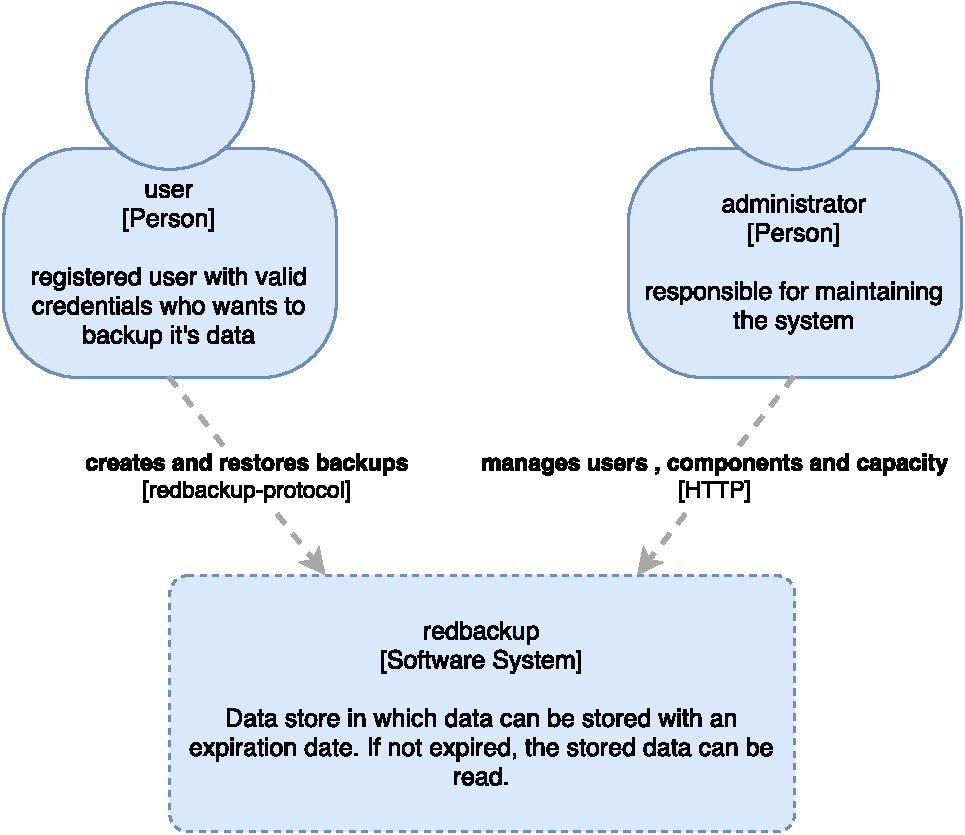
\includegraphics[width=0.5\linewidth]{resources/c4-overview}
	\caption[C4 System Context diagram]{C4 System Context diagram showing the big picture}
	\label{fig:c4-overview}
\end{figure}

The redbackup system consists of four core components as shown in the C4 Container diagram in Figure \ref{fig:c4-container}. A \gls{user} instructs a \gls{client} program running typically on the users machine to perform (unattended) backups and restores.  A client persists and loads its data from one or more interconnected \glspl{node}. A \gls{node} then is in charge of the data and its replication onto other nodes. \Glspl{node} persist the actual data in a separate component, a gls{storage}, to encapsulate persistence from replication and interaction to support different kinds of storage technologies (e.g. plain file systems or databases). A \gls{node} and its \gls{storage} are typically deployed on the same host. One central \gls{management} component orchestrates the configuration of the system by providing metadata, to clients and nodes. This metadata includes a set of all nodes in the system including their addresses and states,  user information and more. Clients and nodes can cache this metadata which ensures that a temporary unavailability of the management component does not compromise the replication and backup process. All components including their responsibilities and interactions are described in more detail in Appendix \fullref{sec:specification}.

\begin{figure}[h]
	\centering
	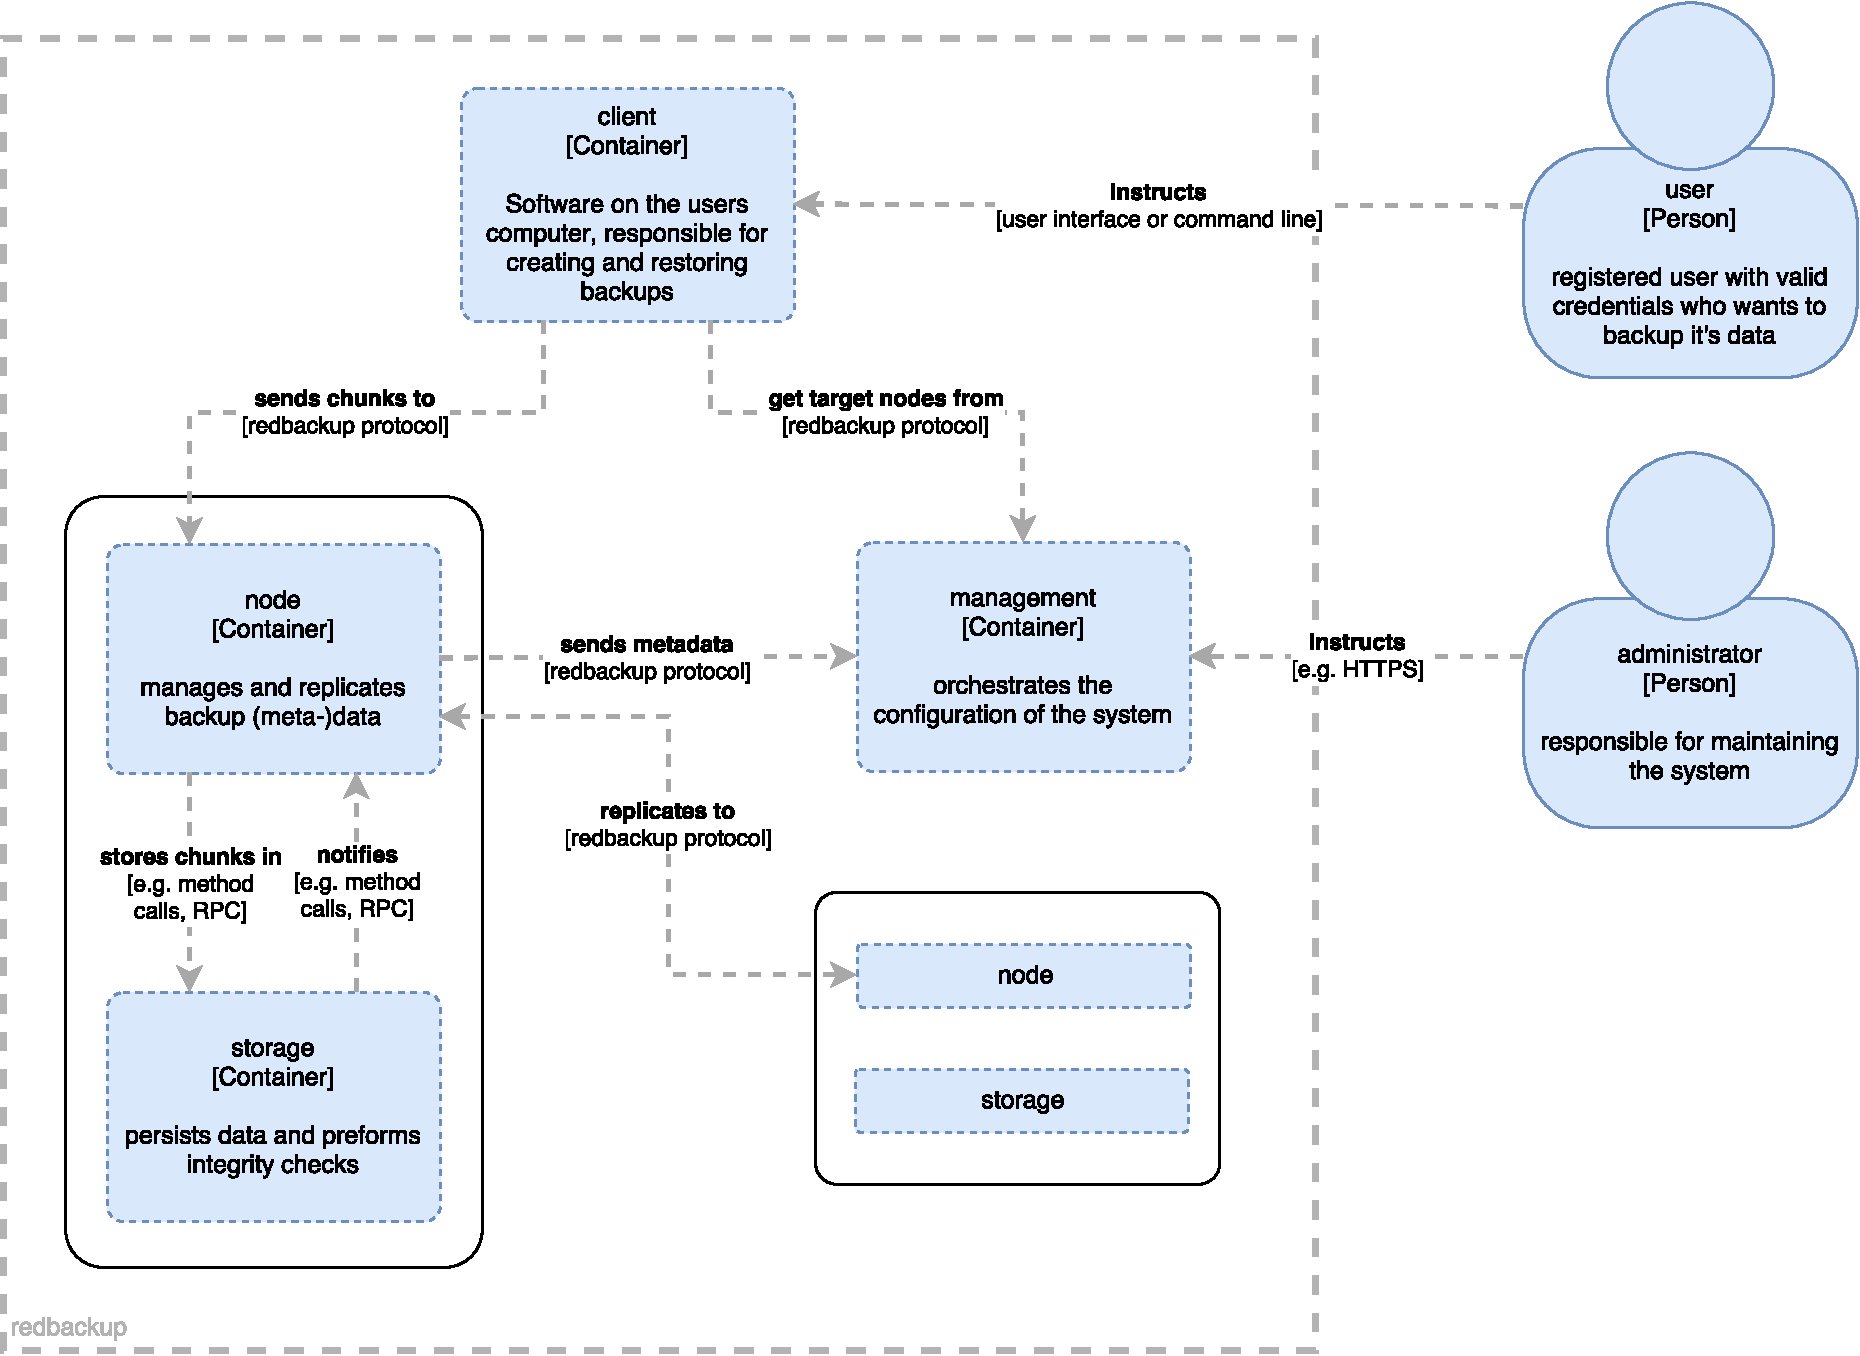
\includegraphics[width=1\linewidth]{resources/c4-container}
	\caption[C4 Container diagram]{C4 Container diagram illustrating the high-level shape of the redbackup software system and how responsibilities are distributed across it.}
	\label{fig:c4-container}
\end{figure}

Redbackup specifies a high-level protocol that is used for internal communication (noted in all C4 diagrams as \emph{redbackup protocol}). We deliberately specified the communication on a high level to encapsulate the underlying protocol. In the prototype, we used a custom, minimal protocol that is based on TCP and sends framed Message Pack\footnote{\url{https://msgpack.org/}} encoded messages. We also encapsulated the (de-) serialisation mechanisms in forwarder and receiver components as specified in the Forwarder Receiver Pattern Pattern \cite{POSA1}.  If we decided to switch to HTTP as the underlying protocol in the future, e.g. to overcome firewall issues, only these forwarder and receiver components have to be adapted while the actual message format does not change. 

\subsection{Replication}
% Planned and unplanned leaving of nodes
% Management down

As for this study project, we only specified n-replication (See \fullref{sec:fundamental-design-decisions}) because it is the most straightforward strategy to implement. A \gls{node} is in charge for all data stored on it. Each \gls{node} - hereafter called \gls{sending-node} -  picks $n$ random data \glspl{chunk} that are stored on it. It then randomly picks one other \gls{node} - hereafter called \gls{designated-node} - and requests which of the chosen data \glspl{chunk} are persisted on it. The \gls{designated-node} returns a subset of the requested \glspl{chunk} that consists of all \glspl{chunk} that are persent on it. Using this response, the \gls{sending-node} sends all missing \glspl{chunk} to the \gls{designated-node} which acknowledges after successful receipt.

\begin{figure}[h]
    \centering
    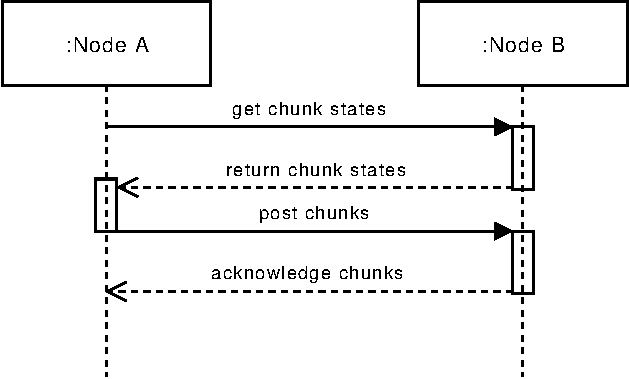
\includegraphics[width=0.6\linewidth]{resources/data_replication.pdf}
    \caption{Data Replication Sequence Diagram}
\end{figure}

This scenario is described in more detail in the appendix \fullref{sec:scenario-data-replication}.

\subsection{Security and Encryption}\label{sec:security-and-encryption}
One of our primary design goals was to ensure that once data is in the redbackup system, it can not be altered or deleted from a \gls{client} to prevent ransomware attacks \cite{young-cryptovirology}. To achieve this, each backup is created with an \gls{expiration-date} on which \glspl{node} are allowed to remove the associated data. Reasoning and potential risks of physical time are discussed in paragraph \fullref{sec:removal-of-old-backups}.

Because \glspl{node} can also be the target of randsomware attacks, each \gls{node}, or its associated \gls{storage} component respectively, must verify that a given data \gls{chunk}s contents are not corrupted using cryptographic hash functions, also known as checksums. To be able to do so, it must be possible to calculate the identifier of such a data \gls{chunk} from its contents. A discussion on the role of hash functions including the chosen algorithms for the study project is carried out in section \fullref{sec:hash-collisions}.

A \gls{client} encrypts backup data \glspl{chunk} when creating a new backup. This ensures that no other participant in the redbackup system can inspect file contents (need-to-know principle \cite{security-patterns}). The encryption and decryption keys are only persisted on the client and must be backed up separately.

All sent \glspl{message} should be signed by the sender. If so, transport layer encryption is not strictly necessary because all user data is already encrypted on the \gls{client} with the only exception of the \gls{expiration-date}.

The \gls{management} component has no knowledge of the persisted data in the system and has only knowledge of the configuration (need-to-know principle \cite{security-patterns}).

A detailed description of these security mechanisms is out of scope for this study project and has to be carried out in the future.

\subsection{Partitioning \& Scaling}

To scale the redbackup system regarding availability and safety more \glspl{node} can be added to the redbackup system. If a given \gls{node} is overloaded, a \gls{client} can use another \gls{node} for its backup creation or restoral. Because both processes require approval of a chosen \gls{node} (See scenarios \fullref{sec:scenario-create-backup} and \fullref{sec:scenario-backup-restore}), an overloaded \gls{node} can finish work in progress backups/restores and reject new requests (following the patterns Finish Work In Progress and Shed Load \cite{fault-tolerance}). The data is replicated to the overloaded \glspl{node} eventually.

Because the proposed system does currently only support \emph{n-replication} (See section \fullref{sec:fundamental-design-decisions}), the maximum storage capacity is the lowest common factor. Therefore, to increase storage capacity, the capacity of all \glspl{node} must be extended to the desired amount.

To minimise network usage deduplication of data is used on the \gls{client}. Deduplication is  discussed in the paragraph Storage Unit in  \fullref{sec:fundamental-design-decisions}.

\subsection{Failure Detection}

Additionally to the above-discussed mechanisms for fault tolerance regarding security and scaling, the following failure detection mechanisms are in place.

Most issues that occur are reported to the \gls{management} component (following the pattern Someone in Charge \cite{fault-tolerance}). The \gls{management} can then decide to notify the system administrator or execute error mitigation processes, e.g. suspend a given \gls{node} temporarily.

If a node tries to connect to another node that is not available, it notifies the management node (following the pattern System Monitor\cite{fault-tolerance}).

Each \gls{node}, or its associated \gls{storage} component respectively, periodically picks $n$ (random) data \gls{chunk} and verifies the persisted contents for possible corruption using the checksum mechanisms discussed in \fullref{sec:security-and-encryption} (following the Pattern Routine Audits \cite{fault-tolerance}). If a corruption is detected, the \gls{storage} notifies the \gls{node} which notifies the \gls{management}.

In case the \gls{management} component is temporarily unavailable, \glspl{node} and \glspl{client} cache configuration data, e.g. which other \glspl{node} exist to perform replication without interruption. Any notifications that were not successfully transmitted to the \gls{management} must be buffered on the \glspl{node} as well to ensure their delivery.

\section{Fundamental Design Decisions}\label{sec:fundamental-design-decisions}

We used the morphological box technique to explore different possible solutions (See Table \ref{tbl:morphological-box})

The chosen option should be as simple as possible for the prototype developed in the study project but extensible for further adaption.

The following paragraphs reason the selected entry in each dimension.

\paragraph{Redundancy}
We originally planned to support \emph{client m-replication}, which means that the client defines a custom degree of redundancy from 1 to the number of nodes. This, however, is a complex mechanism that requires sophisticated algorithms to work correctly and efficiently. For the prototype, we chose the more straightforward to implement option system \emph{n-replication}, where the degree of redundancy for the whole system is equal to the number of nodes in it. Changing this option in the future is hard because it requires fundamental changes in the replication process and the communication protocols.

\paragraph{Storage unit}
The idea of \emph{chunks} come from Borg Backup. Files are partitioned into chunks using a rolling hash which allows deduplication as well as space efficient backups for large files \cite{borg-data-structures}. These are desired properties in a backup system to minimise network and disk usage.

\emph{Encrypting chunks} means that deduplication of the same file coming from different users is not possible anymore but is a necessity for privacy. Encryption is not trivial and requires a user concept that is out of scope of the prototype developed in the study project.
We chose the \emph{plain filesystem} option for the study project to simplify the client implementation. Supporting \emph{encrypted chunks} in the future is possible by just modifying the client.

\paragraph{Role of the management}
The \emph{one in charge} option is the most straightforward option to implement but conflicts with many intentions of the administrator (See \fullref{sec:adminstrator-intention}). We also intended to avoid a single point of failure. We chose the option \emph{autonomous replication} because it guarantees that replication is always ensured and keeps communication relatively simple.

\paragraph{Storage backend}
Using the file system is the simplest possible solution for the study project and therefore selected option. Adding support for other backends in the future is still possible since the storage component is an isolated part of the architecture (See \fullref{sec:component-storage})

The number of files in a folder is limited depending on the used file system, length of a filename and other factors. Some file systems (e.g. ext4) have a global limit for the maximal number of files. This limit is 4 billion files for ext4. \cite{ext4}

We, therefore, use the ext4 file system to persist data in the study project.

\paragraph{Removal of old backups}\label{sec:removal-of-old-backups}
We propose to use a fixed \emph{physical time} that must be specified on backup creation. After expiration, the backup data may be removed by a garbage collector. This may be extended to allow only mutual garbage removal in the future.

A significant problem that \emph{physical time} addresses is the safety of backup data in case a user computer is infected with malware. An illicit application might command the removal of backups, or create new backups to initiate a garbage collection process to free storage capacity.

Nevertheless, the use of \emph{physical time} has the downside of possible data loss due to wrong system times. To lessen this risk, the system should use multiple distinct upstream time-servers. This is given with a high probability, as the proposed redundancy model motivates users to expand the system across multiple physical locations. Furthermore, the client, nodes and management should verify a reasonable accurate time when communicating mutually.

\paragraph{Programming language / ecosystem}
A complete language evaluation can be found in \fullref{sec:language-evaluation}.

\begin{sidewaystable}
	\centering
	\caption[Morphological Box]{Morphological Box}
	\label{tbl:morphological-box}
    \begin{tabu}{X | X X X X}
		\hline
          \textbf{Redundancy}
          & No redundancy
          & Client m-replication: The client defines a custom degree of redundancy (from 1 to the number of nodes).
          & System m-replication: The administrator defines the degree of redundancy for the whole system (from 1 to the number of nodes).
          & \textbf{System n-replication}: The degree of redundancy for the whole system is equal to the amount of nodes in the system.
          \\ \hline

          \textbf{Storage unit}
          & \textbf{Plain files}
          & Encrypted files
          & Chunks: Cut files into multiple parts and store these individually.
          & Encrypted chunks: Same as chunks, but every chunk is individually encrypted.
          \\ \hline


          \textbf{Role of the management}
          & One in charge: The management knows and controls everything (e.g. the location of every file/chunk).
          & Configuration only: The management must be up for administrative tasks only. The nodes are mostly autonomous.
          & \textbf{Autonomous replication}: The management must be available for most of the tasks but replication also works if the management is down.
          & No management: Every node is completely autonomous.
          \\ \hline


          \textbf{Storage backend}
          & \textbf{Plain filesystem}: Just store all files/chunks as files in one directory with a unique identifier.
          & Database: Use an existing database solution (e.g. Git, Redis, RocksDB).
          & Cloud Storage: A proxy to a cloud storage provider (e.g. Amazon S3).
          & Custom: An optimized version of the plain file system option with optimised indexing and compression.
          \\ \hline


          \textbf{Removal of old backups}
          & \textbf{Physical time}: Data is removed on a specified physical time.
          & User command: The user commands removal of data.
          & Free storage: Data is removed, as soon as capacity issues occur.
          & Physical time with mutual agreement: All nodes must agree before data is removed.
          \\ \hline


          \textbf{Programming language / ecosystem}
          & \textbf{Rust}
          & Go
          & Erlang
          & 
          \\ \hline
	\end{tabu}
\end{sidewaystable}

\subsection{Hash Collisions}\label{sec:hash-collisions}
To achieve deduplication and space-efficient backups for large files, as discussed above, a file/chunk identifier must be derived from the actual file/chunk contents. 
A common mechanism used to derive identifiers from binary data are cryptographic hash functions. Most cryptographic hash functions produce a message digest having a fixed size (e.g. SHA-256\cite{sha-256} produces a 256-bit digest) for a message with an arbitrary length, which can theoretically lead to collisions.
Perfect hash functions do not have this property because their input message size is fixed and equal to the size of the resulting message digest. A perfect hash function is not practical in our case due to the large message digests.
With cryptographic hash functions, collisions are possible but unlikely. Assuming that the applied function does produce equally distributed results, the probability can be calculated based on the birthday problem\cite{birthday-attack} as follows, where $p$ is the number of chunks in the system and $n$ the size of the message digests:

\[
P(p, n) = \frac{p^2}{2^{n+1}}
\]

Assuming we have $p=30^{21}$ files/chunks the system (which is equivalent to two billion years of music assuming each chunk has a size of one byte\cite{seagate-zetabyte}) and using the SHA-256 algorithm, the probability of collisions is about $4.72 \cdot 10^{-16}$, which is highly improbable and may therefore be neglected.

If, however, a collision would happen after all, for example, if the used cryptographic hash function is flawed or the unlikely event occurs, it results in data loss.

In theory, we could detect collisions on the client. To do so, every time an identifier is calculated, the client must verify that if a file with the same identifier exists already in the system, it has the exact same contents. If the contents differ, its a collision.This approach requires a lot of network traffic and can slow down the backup process significantly.

Another place to detect collisions is on the node. A node can verify if the contents of a given file/chunk are equal to the contents already present in the system. The downside of this approach is that it requires the client always to send the full contents of every file, which means there is a lot of additional network traffic.

Both of the described approaches for collision detection have significant costs that are not practical.

As for the study project, we use the SHA-256 algorithm\cite{sha-256} and neglect the risk of hash collisions due to its low probability. Nonetheless, we prepare all protocols and components to use an interchangeable mechanism for the calculation and transmission of file/chunk identifiers.

\subsection{Simplifications in this study project}
\subsubsection{Concrete Architecture}

\subsubsection{Client}
\subsubsection{Node}
\section{Testing}\label{testing}
